\documentclass[reqno, 12pt]{article}
\usepackage{amsmath}
\usepackage{amsfonts}
\usepackage{amssymb}
\usepackage{enumerate}
\usepackage{graphicx}
\usepackage{wrapfig}
\usepackage[mathscr]{euscript}
\usepackage{stmaryrd}
\usepackage[normalem]{ulem}
\usepackage{fullpage}
\newcommand{\R}{\mathbb{R}}
\newcommand{\Z}{\mathbb{Z}}
\newcommand{\Q}{\mathbb{Q}}
\newcommand{\N}{\mathbb{N}}
\newcommand{\Lagr}{\mathcal{L}}
\newcommand{\END}{\hspace*{\fill} $\clubsuit$}
\newcommand{\st}{\sout{$\supset$}}
\newcommand{\vx}{ \mathbf{x} }
\newcommand{\vy}{ \mathbf{y} }
\newcommand{\degree}{^\circ}
\graphicspath{graphics}


\title{Functional Analysis Exploration 2}
\author{Zachary Fendler}
\begin{document}
\maketitle
The purpose of the first section is to show uniqueness of the degree function. What I gathered from \textbf{Proposition 1.1} is that if $A \subset \R^n$ is compact and $f: \, A \rightarrow \R^n$ is continuous, then we can extend $f$ (continuously) to $\R^n$ with an inclusion type mapping $\tilde{f}$. To gain some intuition I drew the auxillary function used in the proof for constructing $\tilde{f}$.
\begin{figure}[h]
	\centering
	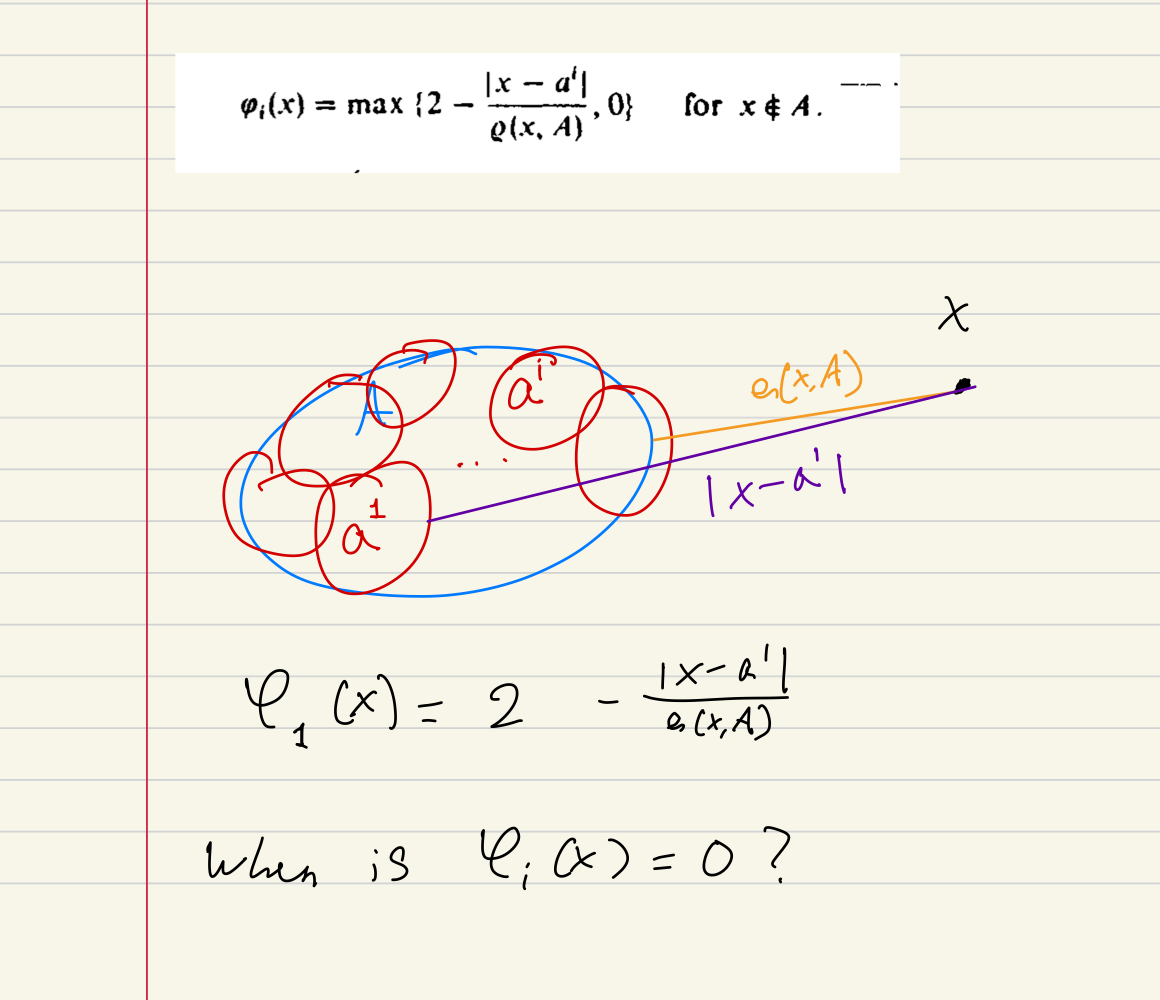
\includegraphics[width = .5\textwidth]{prop1_1-1.jpeg}
	\caption{Illustration of $\varphi_1(x)$.}
\end{figure}
\begin{figure}[h]
	\centering
	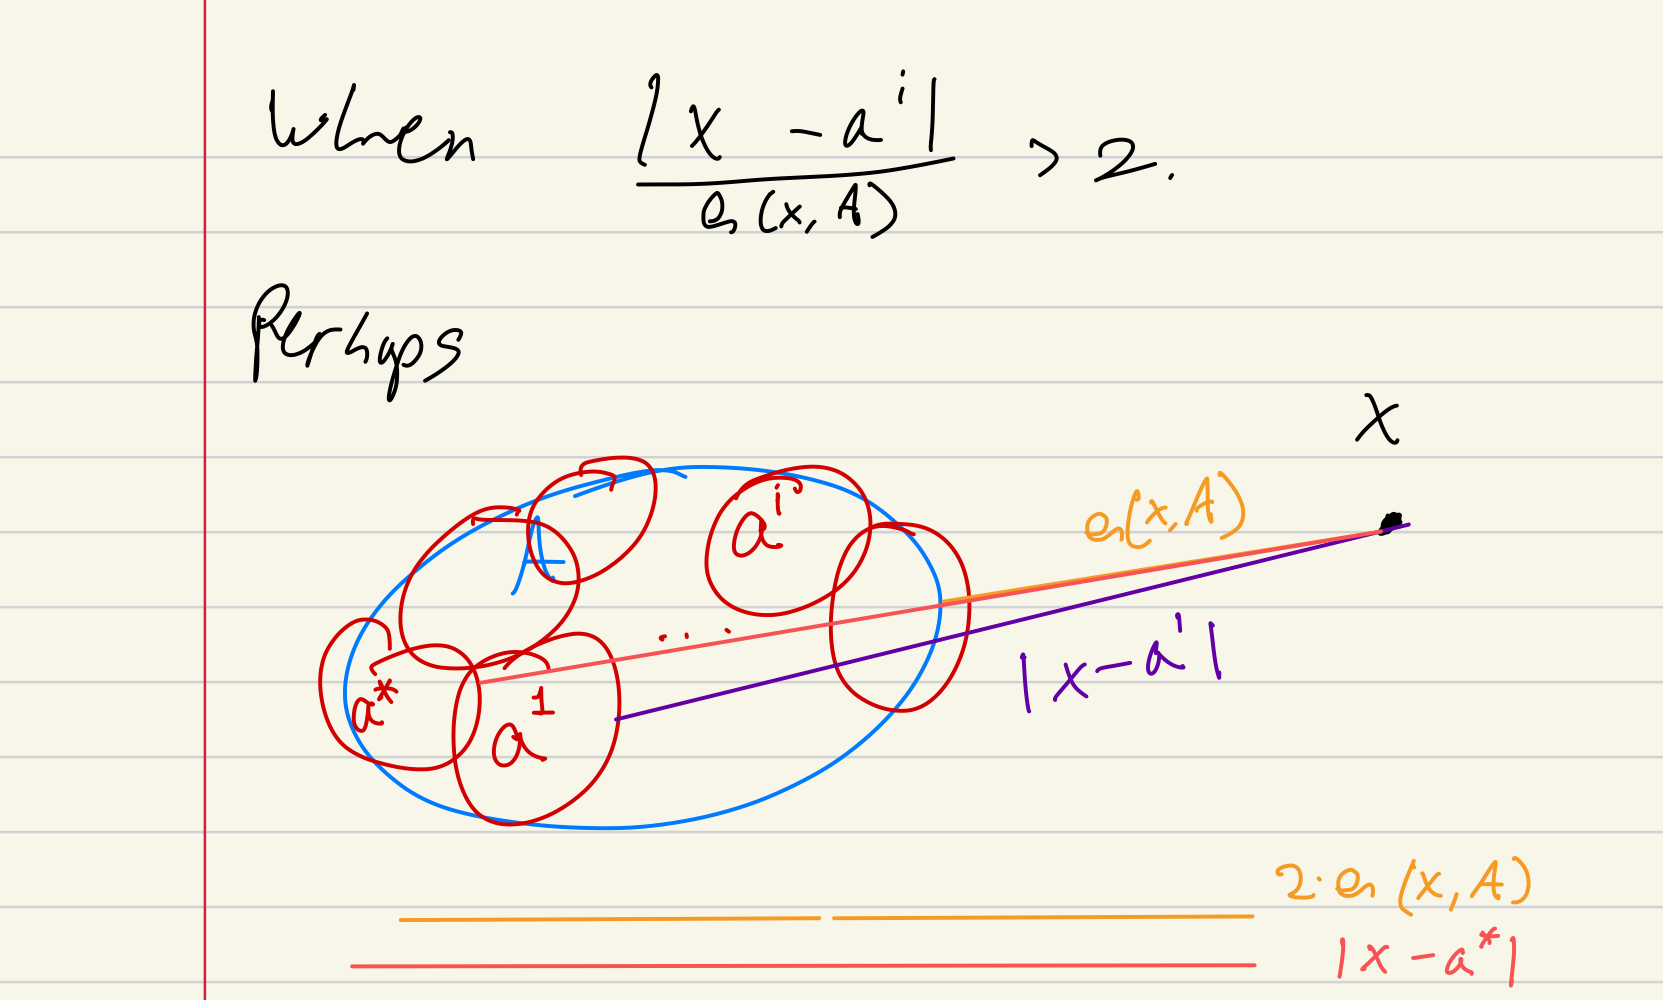
\includegraphics[width = .5\textwidth]{prop1_1-2.jpeg}
	\caption{Illustration of when $\varphi_*(x)=0$.}
\end{figure}
I suspect the $2$ used in the definition is to work out nicely with the definition of $\tilde{f}$ which is
$$\tilde{f}(x) = \begin{cases}
f(x) \qquad &\text{for}\, x \in A \\
\left(\sum_{i\geq 1}2^{-i}\varphi_i(x)\right)^{-1} \sum_{i \geq 1}2^{-i}\varphi_i(x) f(a^i) \qquad &\text{for} \, x \notin A
\end{cases}$$
where $a^i$ is the $i$th subset of the subcover for the compact set $A$. 
The "mollifier" function $\varphi_\alpha : \, \R^n \rightarrow \R$ defined as 
$$\varphi_1 = \begin{cases}
	c\cdot \text{exp}\left(-\frac{1}{1- |x|^2}\right) \qquad &\text{for} \, |x| < 1 \\
	0 \qquad &\text{otherwise}
\end{cases}$$
where $c > 0$ such that $\int_{\R^n}\varphi_1(x) dx = 1$, and $\varphi_\alpha(x) = \alpha^{-n}\varphi_1(x/\alpha)$. This was used in \textbf{Proposition 1.2}.
\begin{figure}
\centering
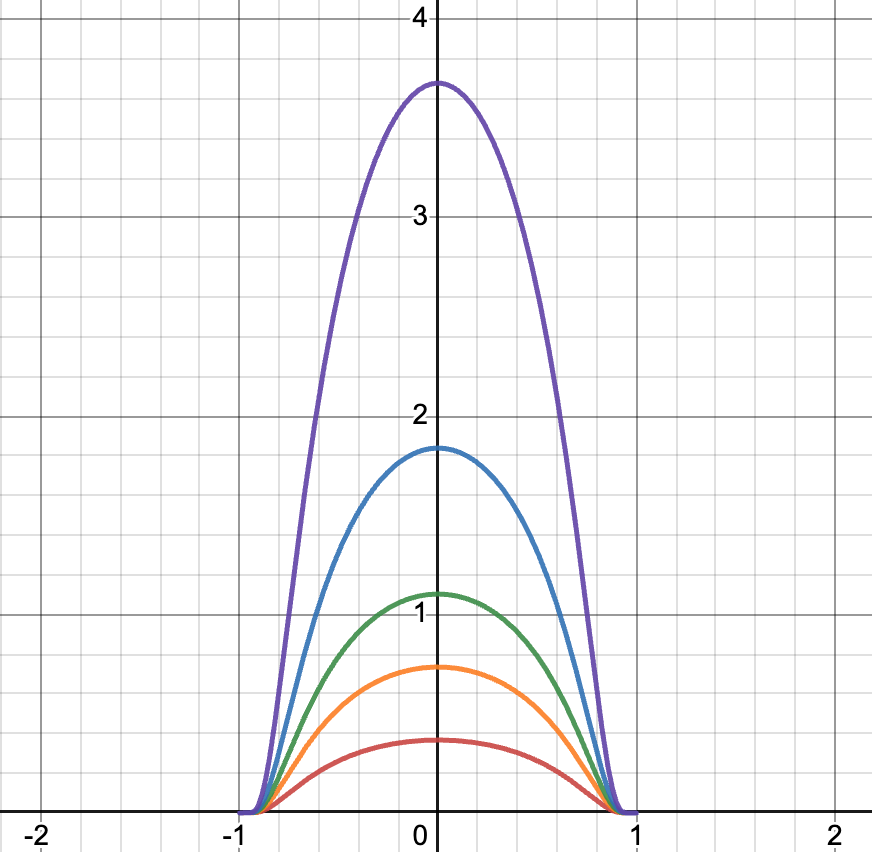
\includegraphics[width = .5\textwidth]{mollifier.png}
\caption{Mollifier function (Deimling page 7) for $c = 1,2,3,5,10$ for curves red, orange, green, blue, and pruple, respectively.}
\end{figure}
Again, I wanted to get an idea of what these functions look like that are used in the proofs. 
\\\\A lot of the proofs this section seemed to come out of thin air and then Deimling will say, "don't worry as a more general proof will be given later in the book." Because of this, I am sort of taking these results at "face value" for now. I noticed there is often another function set up as a convex combination of two functions of interest for some proofs. I wonder if this is a strategy commonly used in homotopy proofs for deformations. \END
\end{document}
